\documentclass[11pt,letterpaper]{article}
\usepackage[utf8]{inputenc}
\usepackage[T1]{fontenc}
\usepackage[provide=*,spanish]{babel}
\usepackage[margin=2.3cm]{geometry}
\usepackage{amsmath,amssymb,booktabs,tabularx,array}
\usepackage{xcolor,tikz,listings,enumitem,hyperref}
\usetikzlibrary{arrows.meta,positioning}
\definecolor{verde}{HTML}{075948}
\hypersetup{colorlinks=true,linkcolor=verde,urlcolor=verde}
\setlength{\parindent}{0pt}
\setlength{\parskip}{6pt}
\setlist{itemsep=3pt,topsep=4pt}
\lstset{basicstyle=\ttfamily\small,breaklines=true,frame=single,columns=fullflexible,keepspaces=true}
\newcommand{\pregunta}[1]{\begin{quote}\color{verde}\textbf{Para pensar:} #1\end{quote}}
\title{\textbf{¿Cómo encontrar un camino sin enumerarlos todos?}\\[4pt]\large Iteración, recurrencia y recursividad\\Dijkstra y el modelo de programación lineal}
\author{Apunte de estudio: Análisis y Diseño de Algoritmos\\UAM Azcapotzalco}
\date{}
\begin{document}
\maketitle

\section{Primero: recurrencia y recursividad no son lo mismo}
Una recurrencia y una implementación recursiva pueden describir el mismo problema, pero no son lo mismo. Primero compara qué representa cada una.

\begin{center}
\begin{tabularx}{\linewidth}{>{\raggedright\arraybackslash}p{2.7cm}XX}
\toprule
Característica & Recurrencia & Recursividad (o recursión)\\
\midrule
¿Qué es? & Una relación matemática entre valores. & Una técnica de programación basada en llamadas de una función a sí misma, directas o indirectas.\\
¿Qué describe? & Cómo un resultado o un costo depende de casos anteriores o más pequeños. & Cómo se ejecuta un procedimiento mediante nuevas llamadas.\\
¿Dónde aparece? & En fórmulas que definen secuencias, soluciones o costos de algoritmos. & En el código o pseudocódigo de un procedimiento.\\
¿Qué necesita para quedar determinada o terminar? & Valores iniciales o condiciones de frontera suficientes para la relación considerada. & Un caso base y que las llamadas avancen hacia él.\\
Ejemplo & $F(0)=1$.\newline $F(n)=nF(n-1)$, para $n\geq1$. & La función \texttt{factorial(n)} llama a \texttt{factorial(n-1)}.\\
¿Obliga a utilizar la otra? & No: puede calcularse mediante ciclos o recursión. & No necesariamente se escribe una ecuación de recurrencia explícita en el programa.\\
\bottomrule
\end{tabularx}
\end{center}

\subsection{Después: recursividad e iteración}
Tanto la recursión como la iteración permiten ejecutar instrucciones repetidamente. La diferencia está en \textbf{cómo se organiza esa repetición y cómo termina}.

\textbf{Recursividad.} Una función se llama a sí misma para continuar el procedimiento. En un algoritmo que debe terminar, esas llamadas necesitan llegar a un \emph{caso base}: una situación que se resuelve sin hacer otra llamada recursiva. Además, cada llamada debe acercarse a ese caso base.

Por ejemplo, \texttt{factorial(4)} necesita \texttt{factorial(3)}, que necesita \texttt{factorial(2)}, y así hasta \texttt{factorial(0)}. En ese momento se devuelve 1; después cada llamada utiliza el resultado de la anterior para completar su multiplicación. No basta con llamar una y otra vez: también hay que entender \textbf{qué se devuelve al regresar}.

\textbf{Iteración.} Un ciclo permite repetir una sentencia o un conjunto de sentencias. La repetición puede continuar mientras una condición sea verdadera, detenerse cuando se cumpla una condición de salida o ejecutarse un número previamente establecido de veces.

Por ejemplo, para calcular el factorial de 4 mediante un ciclo, empezamos con un acumulador igual a 1 y lo multiplicamos sucesivamente por 1, 2, 3 y 4. El ciclo termina al completar esas cuatro repeticiones; ninguna función necesita llamarse a sí misma.

\textbf{Cuidado con la condición de terminación.} No todos los mecanismos repiten ``hasta que una condición sea verdadera'': un \texttt{while} repite mientras su condición sea verdadera y sale cuando es falsa; una función recursiva deja de hacer nuevas llamadas cuando alcanza su caso base. Si el estado no cambia en la dirección necesaria, cualquiera de los dos puede no terminar.

\pregunta{Si una función contiene el caso base $n=0$, pero en cada llamada usa $n+1$ en lugar de $n-1$, ¿llegará a ese caso base al comenzar con $n=4$? ¿Qué falla?}

Por ejemplo, el factorial satisface la recurrencia
\[
F(0)=1,\qquad F(n)=nF(n-1),\quad n\geq1.
\]
Para calcular $F(4)$, la relación permite escribir
\[
F(4)=4F(3)=4\cdot3F(2)=4\cdot3\cdot2F(1)=24.
\]
Esta relación \textbf{no obliga} a usar funciones recursivas. Un ciclo también puede multiplicar $1,2,3,4$.

\pregunta{Si calculas Fibonacci con un ciclo, ¿deja de cumplirse $F_n=F_{n-1}+F_{n-2}$? Explica por qué una recurrencia no es una forma exclusiva de programar.}
En esta sesión estudiaremos un algoritmo \textbf{iterativo}: Dijkstra. Actualizar valores con resultados previos no convierte una implementación en recursiva.

\section{El problema: viajar de Universidad a UAM Azcapotzalco}
Imagina que estás en Universidad y quieres llegar a UAM Azcapotzalco. Estas estaciones pertenecen al \textbf{Metro}. El primer paso no consiste en elegir un algoritmo: consiste en decidir qué queremos mejorar.
\pregunta{¿Qué significa ``mejor camino'': menos conexiones, menos tiempo o menos transbordos? ¿Esos objetivos siempre conducen a la misma ruta?}

En este apunte buscamos el camino de \textbf{menor tiempo total}. Representamos una red como un grafo dirigido $G=(V,E)$:
\begin{itemize}
\item $V$: conjunto de vértices; representan estaciones o estados de viaje.
\item $E$: conjunto de arcos $(u,v)$; representan conexiones permitidas.
\item $c_{uv}$: tiempo de recorrer el arco $(u,v)$, medido en minutos.
\item $s$: origen; $t$: destino.
\end{itemize}
Para distinguir transbordos en una red real, podemos usar un vértice por combinación \emph{estación--línea} y añadir arcos de transbordo. Las dos direcciones de un servicio pueden tener arcos separados y tiempos distintos.

\subsection{Una red pequeña para aprender el procedimiento}
\textbf{La siguiente red es didáctica: tanto las conexiones como los tiempos son ficticios. No representa el mapa real del Metro ni un tiempo real de viaje.} Los símbolos $s$ y $t$ conservan el papel de origen y destino del problema; $a$ y $b$ son puntos intermedios abstractos.

\begin{center}
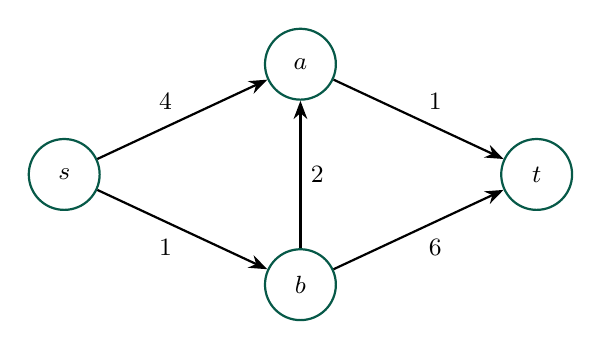
\begin{tikzpicture}[>=Stealth,every node/.style={font=\small},v/.style={circle,draw=verde,thick,minimum size=9mm}]
\node[v] (s) at (0,0) {$s$};
\node[v] (a) at (3,1.4) {$a$};
\node[v] (b) at (3,-1.4) {$b$};
\node[v] (t) at (6,0) {$t$};
\draw[->,thick] (s)--node[above left]{4} (a);
\draw[->,thick] (s)--node[below left]{1} (b);
\draw[->,thick] (b)--node[right]{2} (a);
\draw[->,thick] (a)--node[above right]{1} (t);
\draw[->,thick] (b)--node[below right]{6} (t);
\end{tikzpicture}
\end{center}
\begin{center}
\begin{tabular}{ccc}
\toprule
Arco & Conexión & Tiempo ficticio (min)\\
\midrule
$(s,a)$ & Del origen a $a$ & 4\\
$(s,b)$ & Del origen a $b$ & 1\\
$(b,a)$ & De $b$ a $a$ & 2\\
$(a,t)$ & De $a$ al destino & 1\\
$(b,t)$ & De $b$ al destino & 6\\
\bottomrule
\end{tabular}
\end{center}
En esta red pequeña podemos comprobar tres rutas:
\[
\begin{aligned}
s\to a\to t &: 4+1=5,\\
s\to b\to t &: 1+6=7,\\
s\to b\to a\to t &: 1+2+1=4.
\end{aligned}
\]
La tercera ruta tarda menos aunque usa más arcos. \textbf{Menos conexiones no significa necesariamente menos tiempo.} Enumeramos estas tres rutas solo para comprobar después los resultados; un algoritmo para una red grande debe evitar depender de esa enumeración.

\section{¿Cómo escribir el modelo de programación lineal?}
\subsection{Qué representa cada variable}
Para cada arco definimos $x_{uv}$ como la cantidad de un flujo de viaje de una unidad que enviamos por $(u,v)$. En una solución que representa un camino:
\[
x_{uv}=\begin{cases}1,&\text{si el camino utiliza el arco }(u,v),\\0,&\text{si no lo utiliza.}\end{cases}
\]
Nuestra red tiene cinco variables: $x_{sa},x_{sb},x_{ba},x_{at},x_{bt}$. Por ejemplo, $x_{ba}=1$ significa que usamos la conexión de $b$ a $a$.

\textbf{¿Por qué llamarlo programación lineal si interpretamos ceros y unos?} En el modelo imponemos $x_{uv}\geq0$, no una restricción binaria. La matriz de conservación de flujo de una red tiene una propiedad, llamada \emph{unimodularidad total}, que, con balances enteros, permite obtener soluciones básicas factibles enteras. Para este problema de flujo de una unidad existe una solución óptima que representa un camino; no necesitamos programación entera. Una solución óptima no básica puede repartir flujo entre caminos empatados. Esta propiedad no se conserva automáticamente al añadir cualquier restricción adicional.

\subsection{La función objetivo}
Multiplicamos el tiempo de cada conexión por la variable que indica cuánto flujo la utiliza:
\[
\boxed{\min z=4x_{sa}+x_{sb}+2x_{ba}+x_{at}+6x_{bt}.}
\]
El valor de $z$ se mide en minutos. No representa el número de estaciones.

\subsection{Las restricciones: lo que entra y lo que sale}
Usaremos la convención \textbf{flujo saliente menos flujo entrante}.
\begin{align}
x_{sa}+x_{sb}&=1 &&\text{En $s$ sale una unidad.}\label{eq:s}\\
x_{at}-x_{sa}-x_{ba}&=0 &&\text{En $a$ no se crea ni se pierde flujo.}\label{eq:a}\\
x_{ba}+x_{bt}-x_{sb}&=0 &&\text{En $b$ no se crea ni se pierde flujo.}\label{eq:b}\\
-x_{at}-x_{bt}&=-1 &&\text{En $t$ entra una unidad.}\label{eq:t}
\end{align}
Además,
\[
x_{sa},x_{sb},x_{ba},x_{at},x_{bt}\geq0.
\]
La última igualdad es redundante: sumar las tres primeras produce $x_{at}+x_{bt}=1$. Para resolver con símplex conservamos solo las primeras tres, evitando una fila linealmente dependiente.

Para cualquier red, el modelo tiene la forma
\[
\min\sum_{(u,v)\in E}c_{uv}x_{uv},\qquad
\sum_{v:(u,v)\in E}x_{uv}-\sum_{v:(v,u)\in E}x_{vu}
=\begin{cases}1,&u=s,\\-1,&u=t,\\0,&\text{en otro caso},\end{cases}
\quad x_{uv}\geq0.
\]
\pregunta{Sustituye $x_{sb}=x_{ba}=x_{at}=1$ y las otras variables iguales a cero. ¿Se cumplen todas las restricciones? ¿Cuánto vale $z$?}

\section{¿Cómo lo resolvería el método símplex?}
Símplex trabaja con \textbf{bases} de variables y pasa de una solución básica factible a otra. En un problema de minimización busca una variable no básica que pueda aumentar y disminuir el costo sin violar las restricciones.

Mostraremos el método en forma de \textbf{diccionario}: despejamos las variables básicas en términos de las no básicas. Es el mismo cambio de base que se expresa mediante pivotes en una tabla de símplex.

\subsection{Paso 1: una solución básica factible inicial}
Elegimos la ruta $s\to a\to t$, cuyo costo es 5. Tomamos como básicas $x_{sa},x_{at},x_{ba}$ y como no básicas $x_{sb},x_{bt}$. Despejando las restricciones:
\[
\begin{aligned}
x_{sa}&=1-x_{sb},\\
x_{ba}&=x_{sb}-x_{bt},\\
x_{at}&=1-x_{bt}.
\end{aligned}
\]
Al fijar las no básicas en cero:
\[
x_{sb}=x_{bt}=0,\qquad x_{sa}=1,\quad x_{ba}=0,\quad x_{at}=1.
\]
La solución es factible. $x_{ba}$ es básica pero vale cero; esto se llama \textbf{degeneración} y no invalida la solución.

Sustituimos los despejes en la función objetivo:
\begin{align*}
z&=4(1-x_{sb})+x_{sb}+2(x_{sb}-x_{bt})+(1-x_{bt})+6x_{bt}\\
 &=\boxed{5-x_{sb}+3x_{bt}}.
\end{align*}
Los coeficientes de las variables no básicas se llaman \textbf{costos reducidos}. Aumentar $x_{sb}$ reduciría $z$; aumentar $x_{bt}$ lo incrementaría.

\subsection{Paso 2: elegir la variable que entra}
Entra $x_{sb}$ porque su costo reducido es $-1$. Mantenemos $x_{bt}=0$ y hacemos $x_{sb}=\theta$, con $\theta\geq0$:
\[
x_{sa}=1-\theta,\qquad x_{ba}=\theta,\qquad x_{at}=1.
\]
Para no volver negativa a $x_{sa}$ debemos cumplir $\theta\leq1$. Las otras variables no imponen un límite menor. Por tanto, aumentamos $x_{sb}$ hasta $\theta=1$.

\subsection{Paso 3: cambiar la base}
$x_{sa}$ llega a cero y sale de la base. $x_{sb}$ entra. La nueva solución es
\[
x_{sb}=1,\quad x_{ba}=1,\quad x_{at}=1,\quad x_{sa}=x_{bt}=0.
\]
Representa el camino $s\to b\to a\to t$, con $z=4$.

\subsection{Paso 4: comprobar que ya es óptima}
Despejamos ahora en función de las nuevas variables no básicas $x_{sa}$ y $x_{bt}$:
\[
x_{sb}=1-x_{sa},\quad x_{ba}=1-x_{sa}-x_{bt},\quad x_{at}=1-x_{bt}.
\]
La función objetivo queda
\[
\boxed{z=4+x_{sa}+3x_{bt}.}
\]
Como $x_{sa}\geq0$ y $x_{bt}\geq0$, \textbf{ninguna solución factible puede tener costo menor que 4}. Nuestra solución alcanza 4, por lo que es óptima.
\pregunta{¿Por qué esta última expresión demuestra optimalidad y no solo que encontramos una ruta mejor que la inicial?}

Símplex no enumera todos los caminos: explora soluciones básicas mediante cambios de base. En esta red conocemos una base factible inicial. En un problema general, si no la conocemos, podemos necesitar una fase I o un procedimiento de inicialización.

\section{¿Qué es Dijkstra y qué información conserva?}
Dijkstra es un algoritmo especializado para encontrar caminos de costo mínimo desde un origen cuando \textbf{todos los pesos son no negativos}. Su implementación habitual es iterativa.

En cada vértice $v$ guarda:
\begin{itemize}
\item $d[v]$: menor costo conocido hasta ese momento para llegar desde $s$ hasta $v$.
\item $\operatorname{pred}[v]$: vértice anterior en el camino que produjo ese costo.
\item Si el vértice ya fue \textbf{fijado}: su distancia mínima quedó establecida.
\end{itemize}
Al inicio, $d[s]=0$ y los demás valores son $\infty$. Infinito significa \emph{todavía no conocemos un camino}, no que hayamos demostrado que no existe.

\subsection{La operación central: relajar una conexión}
Si ya conocemos un camino hasta $u$, pasar por el arco $(u,v)$ cuesta
\[
\text{candidato}=d[u]+c_{uv}.
\]
Si este candidato es menor que $d[v]$, actualizamos
\[
d[v]\leftarrow d[u]+c_{uv},\qquad \operatorname{pred}[v]\leftarrow u.
\]
A esta comparación y posible actualización la llamamos \textbf{relajación}.
\pregunta{Si llegar a $u$ cuesta 3 minutos y de $u$ a $v$ cuesta 2, ¿qué valor compararías con $d[v]$? Si $d[v]=4$, ¿debes actualizarlo?}

\subsection{Pseudocódigo: versión sencilla con selección por recorrido}
\textbf{Entradas:} grafo $G$, costos $c$, origen $s$ y destino $t$.\\
\textbf{Salida:} costo mínimo y un camino, o aviso de que el destino no es alcanzable.
\begin{lstlisting}
DIJKSTRA(G, c, s, t)
    para cada vertice v en V:
        d[v] <- infinito
        pred[v] <- NULO
        fijado[v] <- falso
    d[s] <- 0

    mientras exista un vertice no fijado:
        u <- vertice no fijado con menor d[u]
        si d[u] = infinito:
            salir del ciclo
        fijado[u] <- verdadero
        si u = t:
            salir del ciclo

        para cada arco (u, v) que sale de u:
            si fijado[v] = falso:
                candidato <- d[u] + c[u, v]
                si candidato < d[v]:
                    d[v] <- candidato
                    pred[v] <- u

    si d[t] = infinito:
        devolver "No existe camino desde s hasta t"

    camino <- lista vacia
    v <- t
    mientras v != NULO:
        agregar v al inicio de camino
        v <- pred[v]
    devolver d[t], camino
\end{lstlisting}
Este pseudocódigo devuelve \textbf{un} camino óptimo. Si hay empate, la elección depende del orden de procesamiento. Para obtener todos los caminos óptimos hace falta registrar y manejar los empates; no es lo que pide esta versión.

\section{Usar Dijkstra paso a paso en la misma red}
Inicialmente, $d[s]=0$ y $d[a]=d[b]=d[t]=\infty$.
\begin{enumerate}
\item \textbf{Fijamos $s$.} Por sus conexiones, $d[a]=4$ y $d[b]=1$. Los antecedentes de ambos son $s$.
\item \textbf{Fijamos $b$.} Su distancia 1 es la menor de las no fijadas. Para $a$, el candidato es $1+2=3$, mejor que 4: actualizamos $d[a]=3$ y $\operatorname{pred}[a]=b$. Para $t$, obtenemos $1+6=7$ y guardamos a $b$ como antecedente.
\item \textbf{Fijamos $a$.} Su distancia es 3. Para $t$, el candidato es $3+1=4$, mejor que 7: actualizamos $d[t]=4$ y $\operatorname{pred}[t]=a$.
\item \textbf{Fijamos $t$.} Es el vértice no fijado con menor distancia. Podemos detenernos.
\end{enumerate}
\begin{center}
\begin{tabular}{lcccc}
\toprule
Después de procesar & $d[s]$ & $d[a]$ & $d[b]$ & $d[t]$\\
\midrule
Inicialización & 0 & $\infty$ & $\infty$ & $\infty$\\
$s$ & 0 & 4 & 1 & $\infty$\\
$b$ & 0 & 3 & 1 & 7\\
$a$ & 0 & 3 & 1 & 4\\
$t$ & 0 & 3 & 1 & 4\\
\bottomrule
\end{tabular}
\end{center}
Para reconstruir el camino seguimos los antecedentes:
\[
t\leftarrow a\leftarrow b\leftarrow s.
\]
Al invertir ese orden obtenemos
\[
\boxed{s\to b\to a\to t,\qquad \text{costo mínimo}=4\text{ minutos ficticios}.}
\]
\textbf{No debemos detenernos cuando descubrimos por primera vez el destino.} Después de procesar $b$ conocíamos una ruta de costo 7, pero aún faltaba encontrar la de costo 4. La parada segura ocurre cuando seleccionamos y fijamos el destino.

\subsection{¿Por qué podemos fijar una distancia?}
Dijkstra selecciona la menor distancia entre los vértices no fijados. Como los costos no son negativos, continuar desde un vértice con una distancia mayor no puede producir, mediante costos negativos, una reducción inesperada de esa distancia mínima. Esta propiedad sostiene el procedimiento. \textbf{Con pesos negativos no debemos aplicar Dijkstra sin otra justificación.}

\section{Comparar los métodos y elegir según el problema}
\begin{center}
\begin{tabularx}{\linewidth}{lXX}
\toprule
Aspecto & Programación lineal con símplex & Dijkstra\\
\midrule
Representación & Variables por arco y ecuaciones de flujo & Grafo, distancias y antecedentes\\
Paso central & Elegir variable entrante y cambiar la base & Fijar un vértice y relajar conexiones\\
Resultado en el ejemplo & Ruta de costo 4 & La misma ruta de costo 4\\
Enumeración previa & No necesita listar todos los caminos & No necesita listar todos los caminos\\
Uso & Marco general de optimización lineal & Algoritmo especializado para pesos no negativos\\
\bottomrule
\end{tabularx}
\end{center}
La versión sencilla de Dijkstra que busca el mínimo recorriendo los vértices requiere $O(|V|^2+|E|)$ tiempo; en grafos simples se suele expresar como $O(|V|^2)$. Una versión con listas de adyacencia y un montículo binario requiere $O((|V|+|E|)\log |V|)$. El montículo cambia la implementación de la selección, no el problema que resolvemos.

Para un camino mínimo con pesos no negativos, Dijkstra suele ser más directo que montar un modelo general y resolverlo con símplex. Si todos los arcos cuestan lo mismo y queremos minimizar su número, basta una búsqueda en anchura (BFS). Si incorporamos capacidad, múltiples viajeros o restricciones adicionales, conviene reformular el problema; algunas variantes requieren programación entera y ya no se resuelven con el Dijkstra básico.

\pregunta{En nuestra red, la ruta óptima usa tres arcos. ¿Por qué una búsqueda que minimice el número de arcos podría devolver una ruta distinta?}
\pregunta{Identifica el ciclo que hace iterativo al pseudocódigo. ¿Dónde hay una llamada del procedimiento a sí mismo? ¿Una actualización que usa valores anteriores basta para hablar de recursividad?}

\textbf{Distinción final:} la iteración organiza repeticiones; la recursividad organiza llamadas a la misma función; una recurrencia expresa una dependencia matemática. No son tres clases mutuamente excluyentes de algoritmos.

\end{document}
